\documentclass[../cellseek_paper.tex]{subfiles}

\begin{document}

\section{CellSeek GUI: Streamlined Workflow for Cell Tracking}

To make CellSeek accessible to biologists without programming expertise, we developed an intuitive graphical interface that guides users through a supervised cell tracking workflow. The interface transforms complex computer vision algorithms into simple point-and-click operations, allowing researchers to maintain control over analysis quality while benefiting from automated segmentation and tracking capabilities.

\begin{figure}[H]
  \centering
  \begin{tikzpicture}[
    % Define styles
    workflowstep/.style={rectangle, draw, thick, fill=blue!15, minimum width=2.8cm, minimum height=1.2cm, align=center, rounded corners=3pt},
    interactive/.style={rectangle, draw, thick, fill=green!20, minimum width=2.8cm, minimum height=1.2cm, align=center, rounded corners=3pt},
    data/.style={rectangle, draw, thick, fill=orange!15, rounded corners=5pt, minimum height=1cm, align=center},
    arrow/.style={->, >=stealth, thick},
    feedback/.style={<->, >=stealth, thick, red, dashed},
    label/.style={font=\scriptsize\bfseries}
  ]

  % Step 1: Data Import
  \node[workflowstep] (import) at (0,4) {\textbf{Frame Management}\\Import microscopy\\data \& videos};

  % Step 2: Automatic Segmentation
  \node[workflowstep, right=3.5cm of import] (segment) {\textbf{Segmentation}\\Automatic Cellpose-SAM\\processing};

  % Step 3: Interactive Correction
  \node[interactive, below=2cm of segment] (correct) {\textbf{Interactive Correction}\\SAM point-and-click\\refinement};

  % Step 4: Temporal Tracking
  \node[workflowstep, left=3.5cm of correct] (track) {\textbf{Temporal Tracking}\\Frame-by-frame\\cell tracking};

  % Step 5: Analysis & Export
  \node[workflowstep, below=2.2cm of track] (export) {\textbf{Analysis \& Export}\\Results visualization\\and data export};

  % Data flow arrows
  \draw[arrow] (import) -- node[above, label] {Multiple formats} (segment);
  \draw[arrow] (segment) -- node[right, label] {Initial masks} (correct);
  \draw[arrow] (correct) -- node[below, label] {Refined masks} (track);
  \draw[arrow] (track) -- node[left, label] {Tracked cells} (export);

  % Visual feedback indicators
  \node[data, above=0.3cm of segment] (preview1) {Real-time preview};
  \node[data, right=0.3cm of correct] (preview2) {Immediate\\visual feedback};

  % User interaction annotations
  \node[below=2cm of correct, align=left, font=\scriptsize] {
    \textbf{User Interactions:}\\[0.15cm]
    \hspace{0.5em}$\bullet$ Click: Add cell regions\\
    \hspace{0.5em}$\bullet$ Ctrl+Click: Remove regions\\
    \hspace{0.5em}$\bullet$ Drag: Define bounding box
  };

\end{tikzpicture}

  \caption{CellSeek GUI workflow overview. The interface implements a two-stage process: (1) Data Import for loading image sequences, and (2) Frame-by-Frame Analysis combining automatic segmentation, manual correction, and temporal tracking. The workflow emphasizes user supervision at each frame to ensure biological accuracy.}
  \label{fig:gui_workflow}
\end{figure}

\subsection{Workflow Design Philosophy}

The interface follows a frame-by-frame supervision approach that prioritizes accuracy over speed. Rather than processing entire image sequences automatically, users advance through frames manually, reviewing and correcting results at each step. This design ensures that segmentation and tracking errors are caught immediately before they can propagate through the analysis, resulting in higher-quality datasets for downstream analysis.

\subsection{Data Import and Preparation}

\begin{figure}[H]
  \centering
  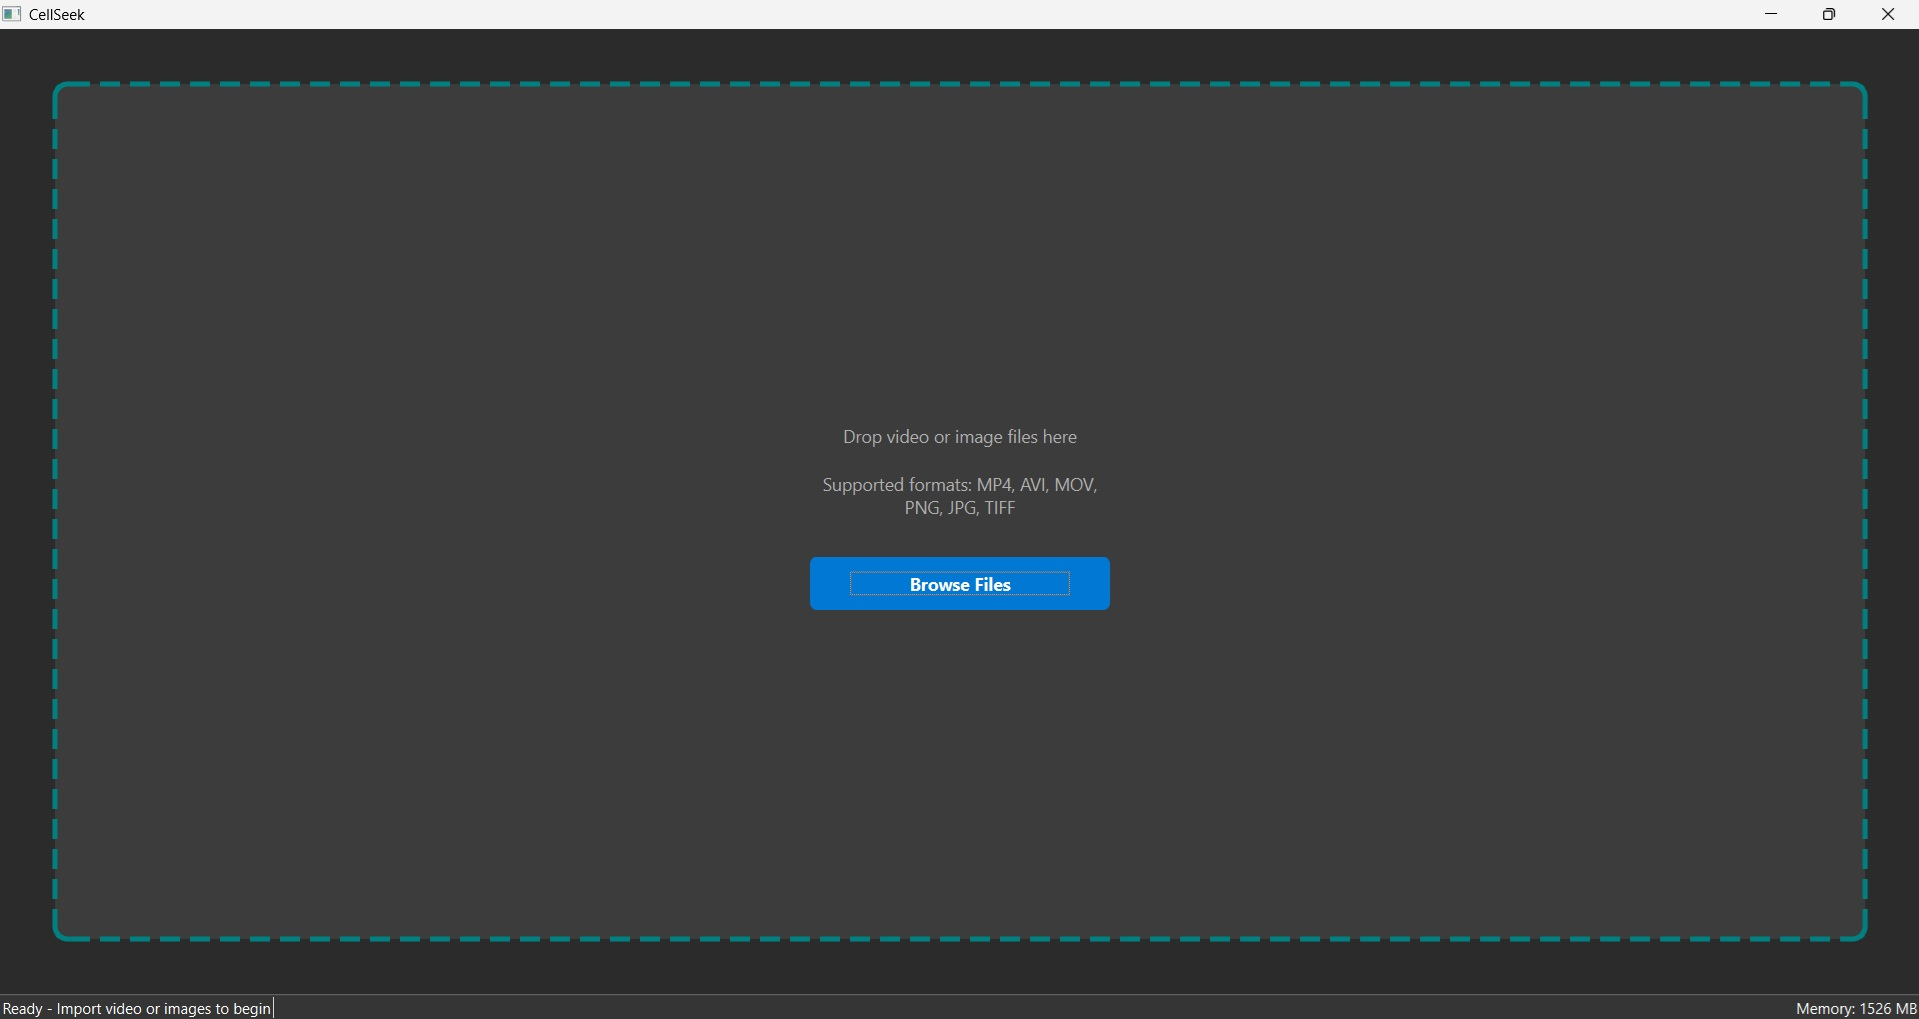
\includegraphics[width=0.8\textwidth]{images/import_images.jpg}
  \caption{Data import interface supporting drag-and-drop functionality for image sequences}
  \label{fig:import_images}
\end{figure}

Users begin by importing their microscopy image sequences through a simple drag-and-drop interface. The system accepts common image formats (PNG, JPEG, TIFF, BMP) and automatically organizes frames in temporal order. This initial step validates data integrity and prepares the sequence for analysis, providing immediate feedback if any files cannot be processed.

\subsection{Automated Initial Segmentation}

\begin{figure}[H]
  \centering
  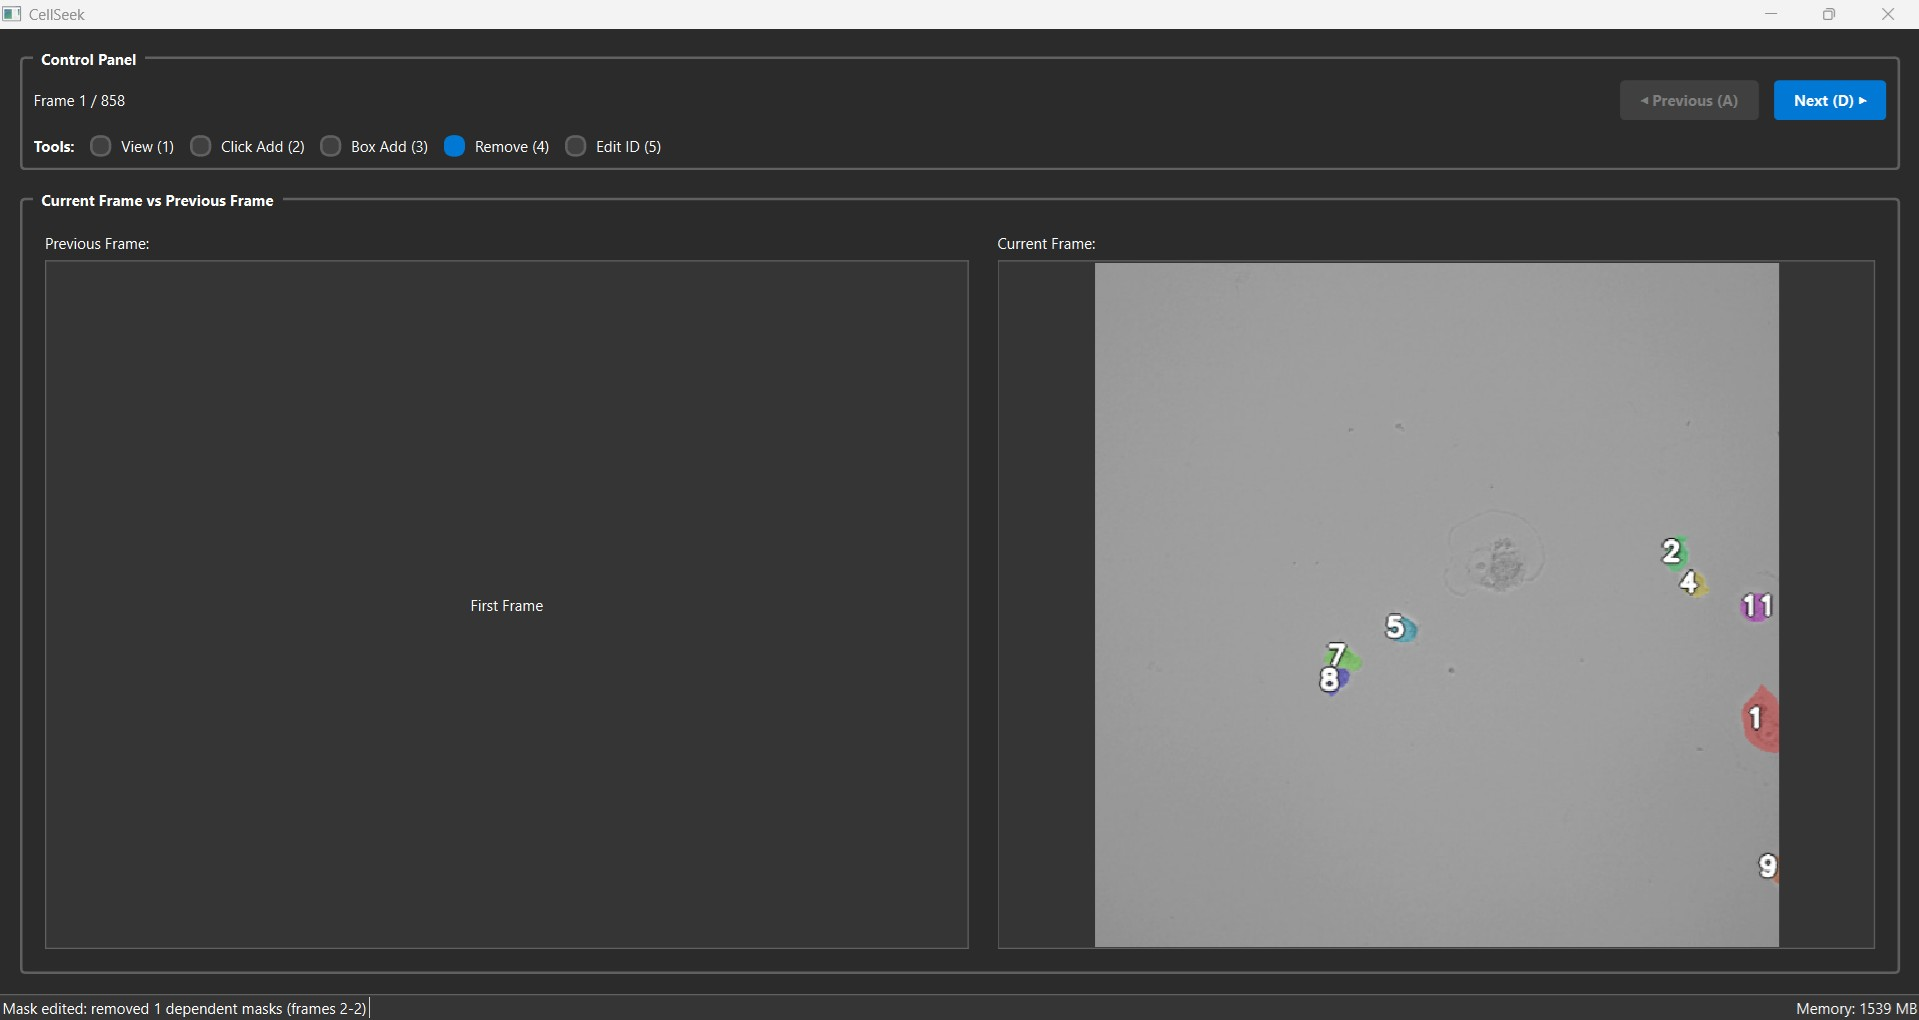
\includegraphics[width=0.8\textwidth]{images/first_frame.jpg}
  \caption{First frame of the microscopy image sequence}
  \label{fig:first_frame}
\end{figure}

The analysis begins with automatic segmentation of the first frame using the CellSAM pipeline. This process requires no user input—simply selecting the first frame triggers automatic cell detection and segmentation. The algorithm identifies individual cells and creates segmentation masks that serve as the foundation for subsequent tracking. Users can immediately see the results overlaid on their image, with each detected cell highlighted in a distinct color.

\subsection{Interactive Correction Tools}

A key strength of CellSeek is the ability to easily correct segmentation errors using intuitive point-and-click tools. The interface provides five interaction modes:

\begin{itemize}
  \item \textbf{View Mode}: Navigate and review segmentation results
  \item \textbf{Click Add}: Click anywhere inside a missed cell to add it to the segmentation
  \item \textbf{Box Add}: Draw a box around a region to segment cells within that area
  \item \textbf{Remove}: Click on incorrectly segmented regions to remove them
  \item \textbf{Edit ID}: Modify cell identities to correct tracking assignments
\end{itemize}

\begin{figure}[H]
  \centering
  \begin{minipage}[b]{0.32\textwidth}
    \centering
    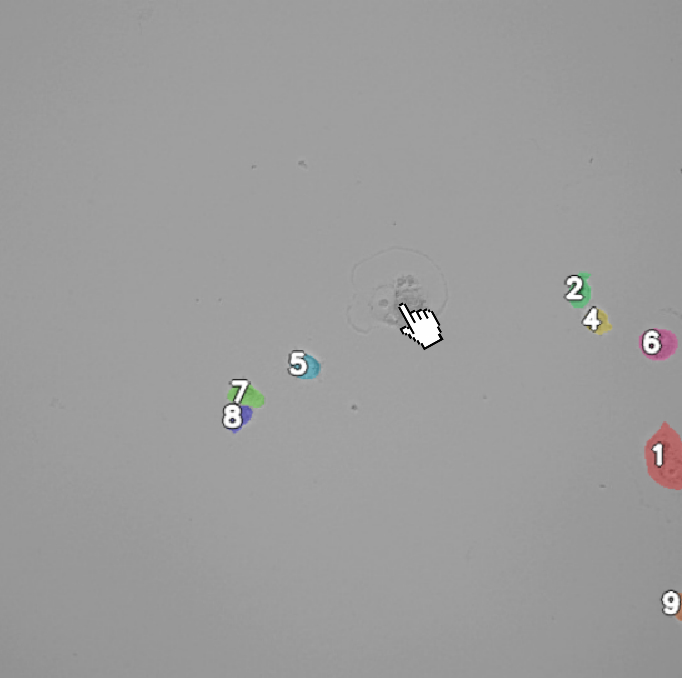
\includegraphics[width=\textwidth]{images/click_on_cell.jpg}
    \caption*{Click Add}
  \end{minipage}
  \hfill
  \begin{minipage}[b]{0.32\textwidth}
    \centering
    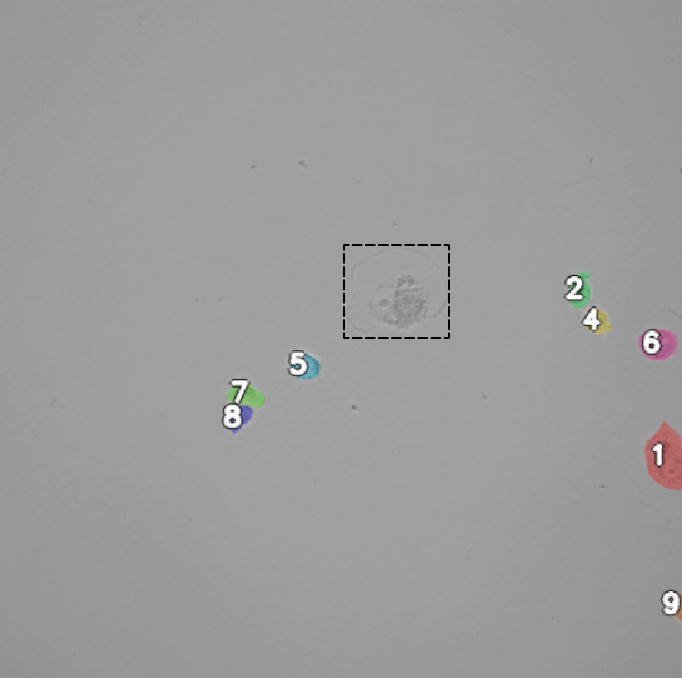
\includegraphics[width=\textwidth]{images/box_on_cell.jpg}
    \caption*{Box Add}
  \end{minipage}
  \hfill
  \begin{minipage}[b]{0.32\textwidth}
    \centering
    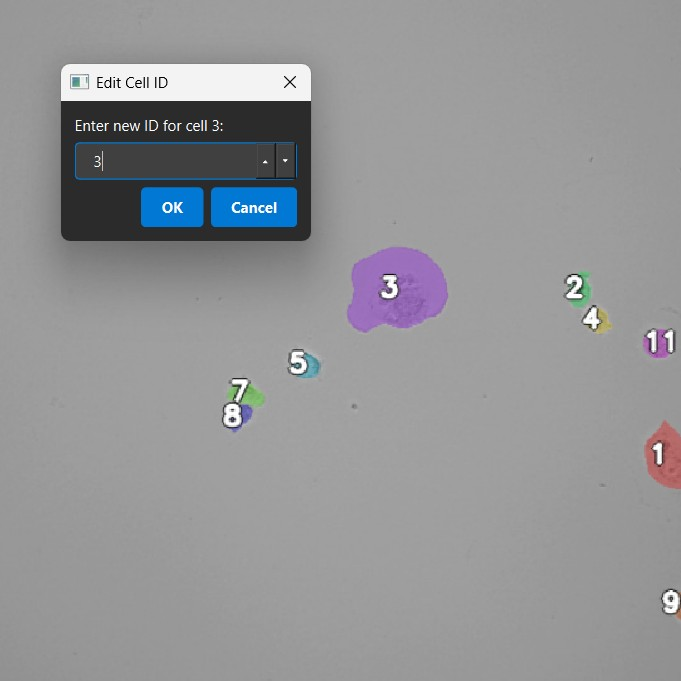
\includegraphics[width=\textwidth]{images/edit_cell_id.jpg}
    \caption*{Edit ID}
  \end{minipage}
  \caption{Examples of interactive correction tools: Click Add, Box Add, and Edit ID.}
  \label{fig:correction_tools}
\end{figure}

These tools utilize the SAM model's interactive capabilities, providing real-time feedback as users make corrections. For instance, when adding a cell, users see a preview of the proposed segmentation before confirming the addition. This immediate feedback allows for rapid and accurate correction of segmentation errors.

\subsection{Frame-by-Frame Tracking Workflow}

\begin{figure}[H]
  \centering
  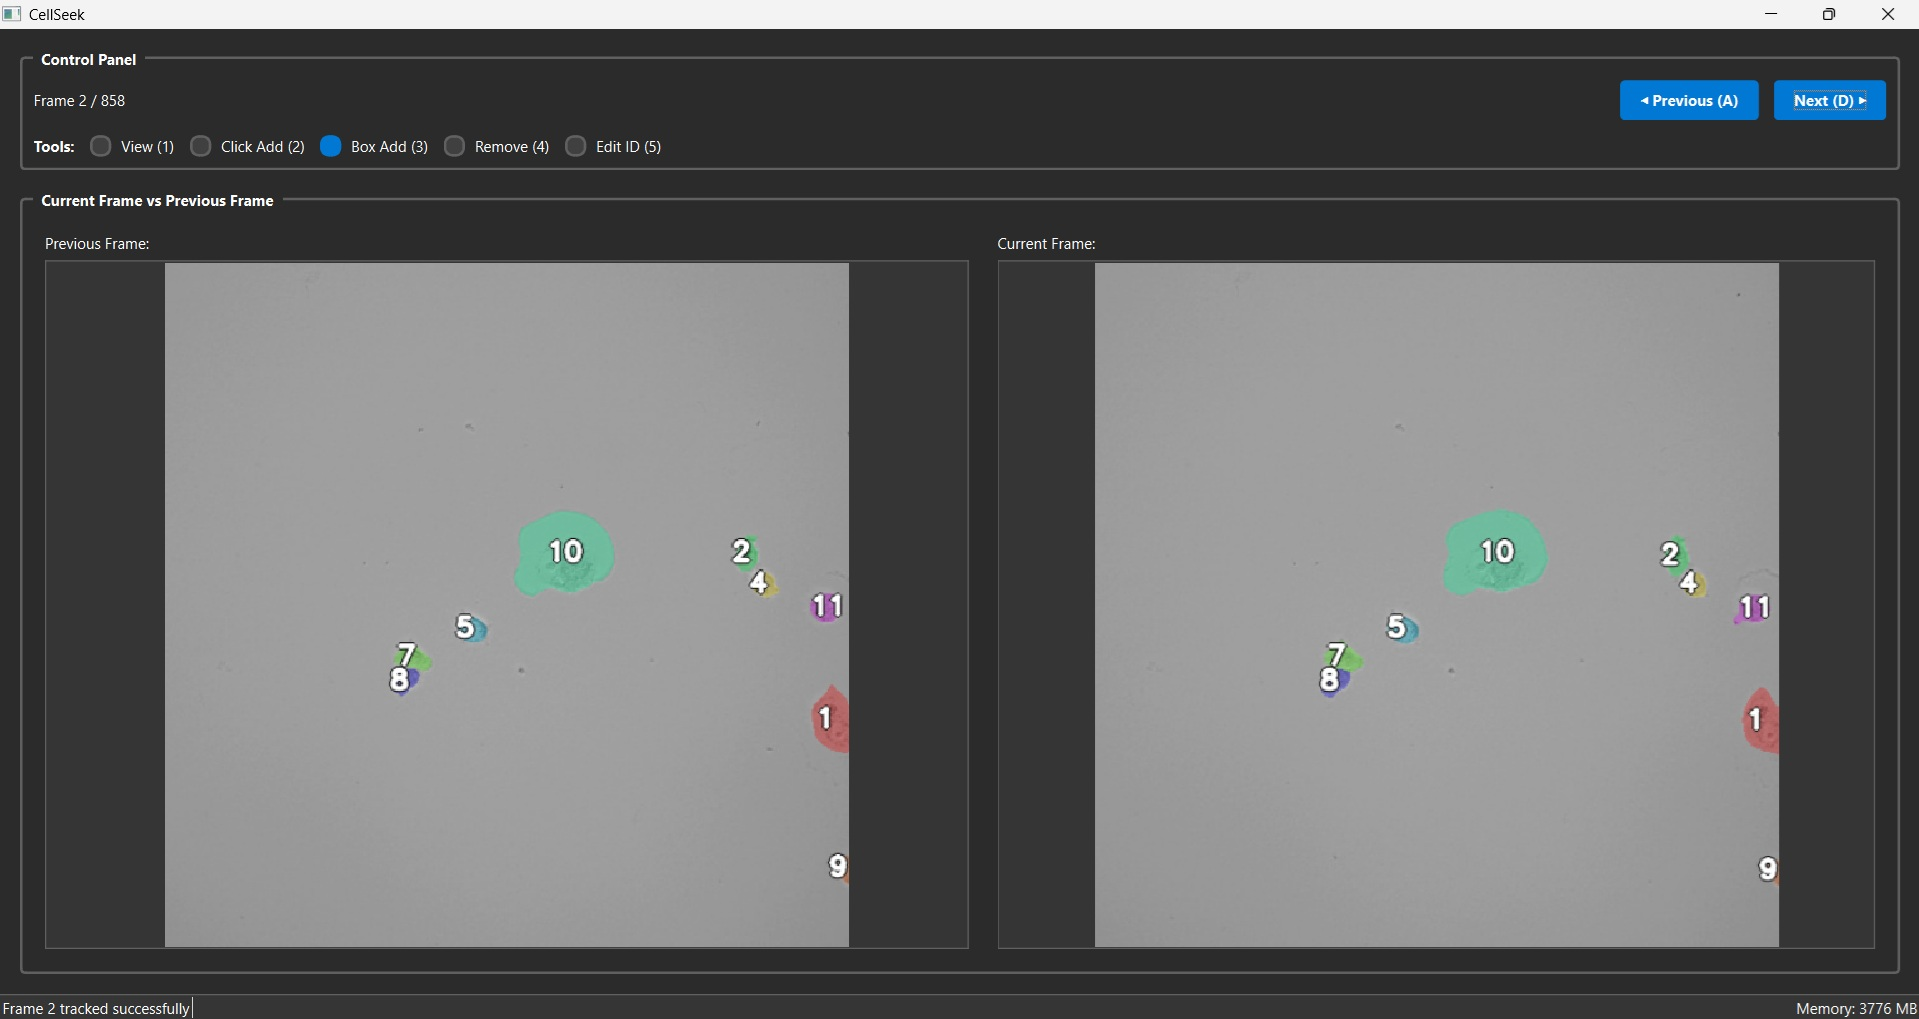
\includegraphics[width=0.8\textwidth]{images/frame_by_frame.jpg}
  \caption{Frame-by-frame tracking workflow}
  \label{fig:frame_by_frame}
\end{figure}

After correcting the first frame's segmentation, users advance through the sequence one frame at a time using simple Previous/Next buttons (or keyboard shortcuts). For each new frame, the system automatically predicts cell positions based on the previous frame using temporal tracking algorithms. Users can immediately see these predictions and make corrections as needed:

\begin{itemize}
  \item \textbf{Automatic Prediction}: The system proposes cell locations in the new frame based on movement patterns from the previous frame
  \item \textbf{Immediate Review}: Users can instantly assess tracking accuracy by comparing predicted positions with actual cell locations
  \item \textbf{Real-time Correction}: Any tracking errors can be corrected immediately using the same interactive tools used for initial segmentation
  \item \textbf{Progressive Refinement}: Each corrected frame becomes the foundation for predicting the next frame, building accuracy over time
\end{itemize}

This supervised approach ensures that tracking errors do not compound throughout the sequence. By catching and correcting mistakes immediately, researchers maintain high-quality tracking data suitable for quantitative analysis.

\subsection{User Experience and Efficiency}

The interface is designed for extended analysis sessions with features that enhance user comfort and efficiency:

\begin{itemize}
  \item \textbf{Dark Theme}: Reduces eye strain during long analysis sessions with microscopy data
  \item \textbf{Keyboard Shortcuts}: Enable rapid navigation and tool switching without mouse movement
  \item \textbf{Visual Feedback}: Immediate updates show the effects of all user actions
  \item \textbf{Memory Monitoring}: Real-time memory usage display helps users manage large datasets
  \item \textbf{Error Prevention}: The system validates user actions and provides clear feedback to prevent common mistakes
\end{itemize}

The frame-by-frame approach, while requiring more user involvement than fully automated methods, provides researchers with complete confidence in their tracking results and enables analysis of challenging datasets where automatic methods might fail.

\end{document}
